\documentclass[border=2mm]{standalone}
\usepackage{tikz}
\usetikzlibrary{calc}

\begin{document}

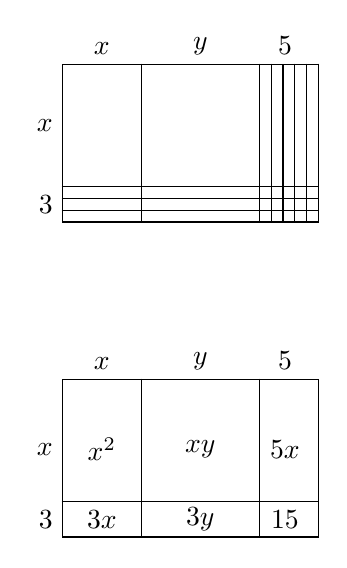
\begin{tikzpicture}[x=1cm,y=1cm,line cap=round]

% --------------------------------------------------
% LƯỚI TRÊN
% --------------------------------------------------

% khung
\draw (1,5) rectangle (4.25,7);
% đường chia hàng, cột
\draw (1,5.15) -- (4.25,5.15);           
\draw (1,5.30) -- (4.25,5.30);           
\draw (1,5.45) -- (4.25,5.45);           
\draw (2,5) -- (2,7);       
\draw (3.5,5) -- (3.5,7);       
\draw (3.65,5) -- (3.65,7);       
\draw (3.80,5) -- (3.80,7);       
\draw (3.95,5) -- (3.95,7);       
\draw (4.10,5) -- (4.10,7);       
\draw (4.25,5) -- (4.25,7);       

% nhãn đầu cột (x, y, 5)
\node at (1.5,7) [above] {$x$};
\node at (2.75,7) [above] {$y$};
\node at (3.825,7) [above] {$5$};

% nhãn đầu hàng (x, 3)
\node at (1,6.225) [left] {$x$};
\node at (1,5.225) [left] {$3$};

% --------------------------------------------------
% LƯỚI DƯỚI (bảng có kết quả)
% --------------------------------------------------

% khung
\draw (1,1) rectangle (4.25,3);
% chia hàng, cột
\draw (1,1.45) -- (4.25,1.45);           
\draw (2,1) -- (2,3);       % chia x / y
\draw (3.5,1) -- (3.5,3);         % chia y / 5

% nhãn đầu cột
\node at (1.5,3) [above] {$x$};
\node at (2.75,3) [above] {$y$};
\node at (3.825,3) [above] {$5$};

% nhãn đầu hàng
\node at (1,2.1125) [left] {$x$};
\node at (1,1.225) [left] {$3$};

% nhãn trong ô
\node at (1.5,2.1125) {$x^{2}$};
\node at (2.75,2.1125) {$xy$};
\node at (3.825,2.1125)  {$5x$};

\node at (1.5,1.225) {$3x$};
\node at (2.75,1.225) {$3y$};
\node at (3.825,1.225)  {$15$};

\end{tikzpicture}


\end{document}